\documentclass[../main.tex]{subfiles}

\begin{document}
\section{Problemas Lineales}
% Esta subsección no estoy seguro si se deberia mantener...
\subsection{Ejemplos de Problemas Lineales}
\subsubsection{Problema del transporte}
Se considera el transporte de un bien desde el productor a los clientes.\\
\begin{minipage}[t]{.45\textwidth}
  \begin{itemize}
    \item El productor tiene $n$ plantas de producción. Cada planta $i \in \{ 1, \ldots, n \}$ ofrece una cantidad $s_i$ de unidades.
    \item Existen $m$ clientes. Cada cliente $j \in \{ 1, \ldots, m \}$ demanda una cantidad $d_j$ de unidades.
    \item El costo por unidad de bien transportado desde la planta $i$ hasta el cliente $j$ es $c_{ij}$.
    \item Toda la demanda debe ser satisfecha.
    \item El objetivo es minimizar el costo total.
  \end{itemize}
\end{minipage}
\hfill
\begin{minipage}[t]{.45\textwidth}
  $x_{ij}$ corresponde a las unidades a transportar desde la planta $i$ hasta el cliente $j$
  \begin{gather*}
    \min \sum_{i \in N, j \in M} c_{ij} x_{ij} \\
    \text{donde } N = \{ 1, \ldots, n \},\ M = \{ 1, \ldots, m \}\\
    s.a.\\
    \sum_{j \in M} x_{ij} \leq s_i \quad \forall i \in N\\
    \sum_{i \in N} x_{ij} \geq d_j \quad \forall j \in M\\
    x_{ij} \geq 0 \quad \forall i \in N, \forall j \in M
  \end{gather*}
\end{minipage}

\subsubsection{Problema de producción e inventario}
Se considera una empresa productora que tiene un horizonte de planificación de $T$ meses para la producción de un bien.\\
\begin{minipage}[t]{.45\textwidth}
  \begin{itemize}
    \item Se considera un costo $c_t$ por producir una unidad del bien en el mes $t \in \{ 1, \ldots, T \}$.
    \item La capacidad productiva del mes $t$ es $K_t$.
    \item Tenemos que satisfacer una demanda de $d_t$ unidades para cada mes $t$.
    \item Es posible guardar productos en bodega desde el mes $t$ al mes $t+1$ con un costo de $h_t$. No hay inventario inicial.
    \item El objetivo es minimizar el costo total.
  \end{itemize}
\end{minipage}
\hfill
\begin{minipage}[t]{.45\textwidth}
  $x_t$ corresponde a las unidades a producir en el mes $t$.

  $y_t$ corresponde a las unidades que se dejarán en la bodega desde el mes $t$ al mes $t+1$.
  \begin{gather*}
    \min \sum_{t \in H} c_t x_t + \sum_{t \in H} h_t y_t \quad \text{donde } H = \{ 1, \ldots, T \}\\
    s.a \\
    x_t \leq K_t \quad \forall t \in H \\
    y_{t-1} + x_t = d_t + y_t \quad \forall t \in H \\
    y_0 = y_T = 0 \\
    x_t, y_t \geq 0 \quad \forall t \in H
  \end{gather*}
\end{minipage}


\subsection{Ejemplos de Problemas Lineales Enteros}
\subsubsection{Problema de la mochila (Knapsack)}
\begin{minipage}[t]{.45\textwidth}
  \begin{itemize}
    \item Se tiene una mochila con capacidad $W$ (kg).
    \item Se tienen $n$ posibles items que se pueden llevar.
    \item Cada item $i \in N = \{ 1, \ldots, n \}$ tiene un peso de $w_i$ (kg) y una utilidad / ganancia de $v_i$ (\$).
    \item El objetivo es maximizar la utilidad de la mochila, pero sin exceder el peso máximo.
  \end{itemize}
\end{minipage}
\hfill
\begin{minipage}[t]{.45\textwidth}
  $x_i$ indica si se lleva el ítem $i$ ($x_i = 1$) o si no se lleva ($x_i = 0$).
  \begin{gather*}
    \max \sum_{i \in N} v_i x_i \\
    s.a. \\
    \sum_{i \in N} w_i x_i \leq W \\
    x_i \in \{ 0, 1 \} \quad \forall i \in N
  \end{gather*}
\end{minipage}

\subsubsection{Problema de asignación}
\begin{minipage}[t]{.45\textwidth}
  \begin{itemize}
    \item Se tiene $n$ tareas que se deben realizar.
    \item Se cuenta con $m$ maquinas que pueden realizar dichas tareas.
    \item Cada una de las máquinas puede realizar a lo más una tarea.
    \item El costo de realizar la tarea $i \in N = \{ 1, \ldots n \}$ en la máquina $j \in M = \{ 1, \ldots m \}$ es $c_{ij}$.
    \item El objetivo es minimizar el costo total de realizar todas las tareas.\footnotemark{}
  \end{itemize}
\end{minipage}
\footnotetext{Observación: Para que esto sea factible, se debe cumplir que $m \geq n$}
\hfill
\begin{minipage}[t]{.45\textwidth}
  $x_{ij}$ indica si se asigna la tarea $i$ a la máquina $j$.
  \begin{gather*}
    \min \sum_{i \in N, j \in M} c_{ij} x_{ij} \\
    s.a. \\
    \sum_{j \in M} x_{ij} = 1 \quad \forall i \in N \\
    \sum_{i \in N} x_{ij} \leq 1 \quad \forall j \in M \\
    x_{ij} \in \{0, 1\} \quad \forall i \in N, \forall j \in M
  \end{gather*}
\end{minipage}

\subsubsection{Problema del vendedor viajero}
\begin{itemize}
  \item Un vendedor desea visitar $n$ ciudades exactamente una sola vez en un tour.
  \item El tiempo que se demora en viajar desde la ciudad $i \in N = \{ 1, \ldots, n \}$ a la ciudad $j \in N$ es $t_{ij}(s)$.
  \item El objetivo es minimizar el tiempo total de viaje.
\end{itemize}


\begin{figure}[h]
  \begin{tikzpicture}
    \node (a) at (2, 1) {a};
    \node (b) at (3, 4) {b};
    \node (c) at (3, 2) {c};
    \node (d) at (1, 2) {d};
    \node (e) at (2, 3) {e};
  \end{tikzpicture}
  \hfill
  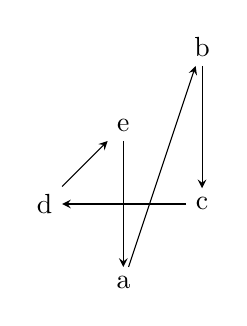
\begin{tikzpicture}
    \node (a) at (2, 1) {a};
    \node (b) at (3, 4) {b};
    \node (c) at (3, 2) {c};
    \node (d) at (1, 2) {d};
    \node (e) at (2, 3) {e};
  
    \draw [-stealth] (a) -- (b);
    \draw [-stealth] (b) -- (c);
    \draw [-stealth] (c) -- (d);
    \draw [-stealth] (d) -- (e);
    \draw [-stealth] (e) -- (a);
  \end{tikzpicture}
  \hfill
  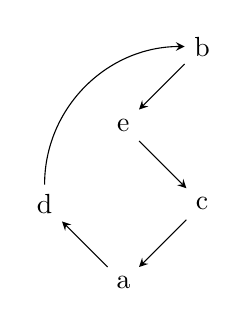
\begin{tikzpicture}
    \node (a) at (2, 1) {a};
    \node (b) at (3, 4) {b};
    \node (c) at (3, 2) {c};
    \node (d) at (1, 2) {d};
    \node (e) at (2, 3) {e};
  
    \draw [-stealth] (a) -- (d);
    \draw [-stealth] (d) to[out=90, in=180, looseness=1] (b);
    \draw [-stealth] (b) -- (e);
    \draw [-stealth] (e) -- (c);
    \draw [-stealth] (c) -- (a);
  \end{tikzpicture}
  \caption{Distintos tours posibles para las ciudades $a$, $b$, $c$, $d$ y $e$.}
\end{figure}

$x_{ij}$ corresponde a si el camino entre la ciudad $i$ y la ciudad $j$ existe en el tour.
\begin{gather*}
  \min \sum_{i \in N, j \in N} t_{ij} x_{ij} \\
  s.a. \\
  \sum_{j \in N} x_{ij} = 1 \quad \forall i \in N \\
  \sum_{i \in N} x_{ij} = 1 \quad \forall j \in N \\
  x_{ii} = 0 \quad \forall i \in N \\
  x_{ij} \in \{ 0,1 \} \quad \forall i \in N , \forall j \in N
\end{gather*}

Si bien el modelamiento es correcto, no se está considerando un detalle importante: ¿Qué pasa con los subtours o subcíclos?

\begin{figure}[h]
  \centering
  \begin{tikzpicture}
    \node (a) at (2, 1) {a};
    \node (b) at (3, 4) {b};
    \node (c) at (3, 2) {c};
    \node (d) at (1, 2) {d};
    \node (e) at (2, 3) {e};
    \node (f) at (1, 1) {f};
  
    \draw [-stealth] (a) -- (f);
    \draw [-stealth] (f) -- (d);
    \draw [-stealth] (d) -- (a);

    \draw [-stealth] (b) -- (e);
    \draw [-stealth] (e) -- (c);
    \draw [-stealth] (c) -- (b);
  \end{tikzpicture}
  \caption{Un caso de existencia de subtours / subcíclos}
\end{figure}

Es necesario corregir esto. 

$x_{ij}$ corresponde a si el camino entre la ciudad $i$ y la ciudad $j$ existe en el tour.
\begin{gather*}
  \min \sum_{i \in N, j \in N} t_{ij} x_{ij} \\
  s.a. \\
  \sum_{j \in N} x_{ij} = 1 \quad \forall i \in N \\
  \sum_{i \in N} x_{ij} = 1 \quad \forall j \in N \\
  x_{ii} = 0 \quad \forall i \in N \\
  {\color{red} \sum_{i \in S, j \in S} x_{ij} \leq |S| - 1 \quad \forall S \subseteq N : 2 \leq |S| \leq n - 1} \\
  x_{ij} \in \{ 0,1 \} \quad \forall i \in N , \forall j \in N
\end{gather*}


\section{Operadores Lógicos}
\subsection[AND]{``y'' lógico / AND / $\wedge$}
El operador lógico ``AND'' significa que para que se cumpla la condición (en otras palabras, devolver \texttt{true}), es necesario que se cumplan las dos condiciones unidas con $\wedge$.

\begin{minipage}[t]{.45\textwidth}
  Escritura lógica:
  \begin{gather*}
    x_{ij} = 1 \Leftrightarrow y_i = 1 \wedge y_j = 1  
  \end{gather*}

  Esto significa: $x_{ij}$ es $1$ si y solo si $y_i = 1$ y $y_j = 1$. Si una de las dos condiciones no se cumple, $x_{ij} \not= 1$.
\end{minipage}
\hfill
\begin{minipage}[t]{.45\textwidth}
  Modelamiento lineal:
  \begin{gather*}
    x_{ij} \leq y_i \\
    x_{ij} \leq y_j \\
    y_i + y_j \leq 1 + x_{ij}
  \end{gather*}
\end{minipage}

\subsection[OR]{``o'' lógico / OR / $\vee$}
El operador lógico ``OR'' significa que para que se cumpla la condición final, basta con que se cumpla al menos una de las condiciones unidas por $\vee$.

\begin{minipage}[t]{.45\textwidth}
  Escritura lógica:
  \begin{gather*}
    x_{ij} = 1 \Leftrightarrow y_i = 1 \vee y_j = 1  
  \end{gather*}

  Esto significa: $x_{ij}$ es $1$ si y solo si $y_i = 1$, $y_j = 1$ o si $y_i = 1$ y $y_j = 1$. Si no se cumple ninguna de las condiciones, $x_{ij} \not= 1$.
\end{minipage}
\hfill
\begin{minipage}[t]{.45\textwidth}
  Modelamiento lineal:
  \begin{gather*}
    y_i \leq x_{ij} \\
    y_j \leq x_{ij} \\
    x_{ij} \leq y_i + y_j
  \end{gather*}
\end{minipage}

\subsection[XOR]{``o'' lógico excluyente / XOR / $\veebar$}
El operador lógico ``XOR'' significa que para que se cumpla la condición final, es necesario que se cumpla solo una de las condiciones unidas por $\veebar$.

\begin{minipage}[t]{.45\textwidth}
  Escritura lógica:
  \begin{gather*}
    x_{ij} = 1 \Leftrightarrow y_i = 1 \veebar y_j = 1 \\
    x_{ij} = 1 \Leftrightarrow (y_i = 0 \wedge y_j = 1) \vee (y_i = 1 \wedge y_j = 0) \\
    x_{ij} = 1 \Leftrightarrow y_i \not= y_j
  \end{gather*}

  Esto significa: $s_{ij}$ es $1$ si y solo si $y_i = 1$ o si $y_j = 1$. Si se cumplen ambas o no se cumple ninguna, $x_{ij} \not= 1$.
\end{minipage}
\hfill
\begin{minipage}[t]{.45\textwidth}
  Modelamiento lineal:
  \begin{gather*}
    x_{ij} \leq y_i + y_j \\
    x_{ij} \leq 2 - y_i - y_j \\
    y_i - y_j \leq x_{ij} \\
    y_j - y_i \leq x_{ij}
  \end{gather*}
\end{minipage}



\end{document}